%!TEX root = ../dokumentation.tex

\chapter{Routes}
\label{ch:Routes}

Die Routes beschreiben die URL-Pfade eines Servers die eine Anwendung aufrufen kann um eine Anfrage zu starten.
Der erste Einstiegspunkt der vorliegenden Anwendung ist - wie in der package.json beschrieben - die index.js Datei.

\begin{figure}[h]
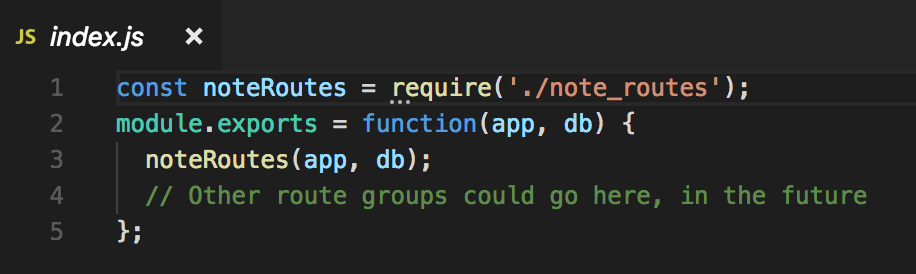
\includegraphics[height=.3\textwidth]{Serverindex.png}
\vspace{3pt}
\caption{Schaubild\footnotemark}
\label{fig:blueant}
\end{figure}

Wie in der ersten Zeile des Codesnippets beschrieben, importiert diese Datei eine weitere Datei namens note\_routes.js. Diese beinhaltet weitere Pfade die weitere API's zur verfügung stellt.

\begin{figure}[h]
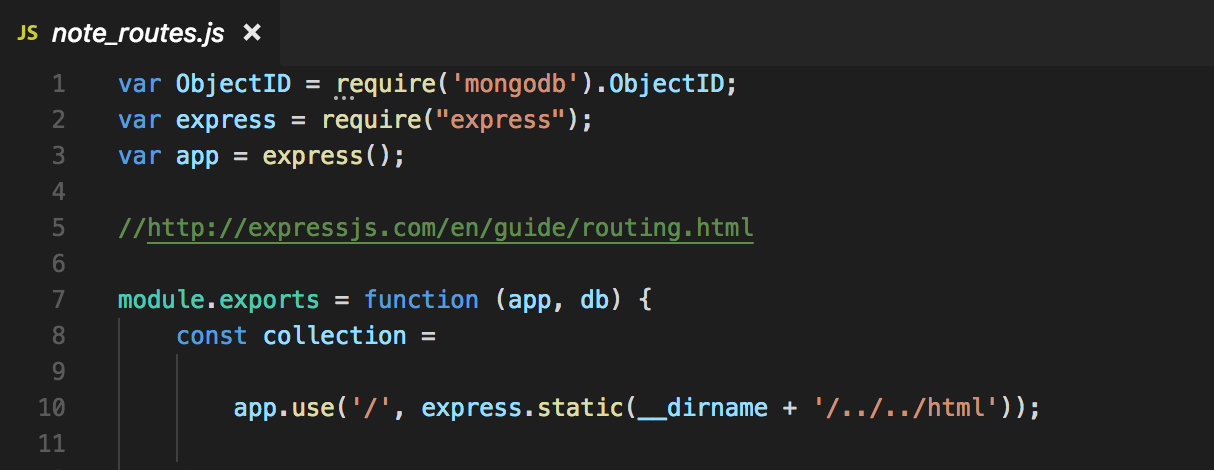
\includegraphics[height=.4\textwidth]{Routesmain.png}
\vspace{3pt}
\caption{Schaubild\footnotemark}
\label{fig:blueant}
\end{figure}


Die note\_routes.js Datei beinhaltet die grundlegenden Verbindungen zur Mongo-Datenbank und dem Express-Framework. Durch diese haben die hier verzeichneten Routes die möglichkeit Requests zu verarbeiten und mit der Datenbank zu interagieren.

Die erste Route beschreibt das Verhalten für einen Request an die URL "/". Die darauf folgende Reaktion ist die Auslieferung der Dateien die sich im übergeordneten Ordner html (Vgl Ordnerstruktur) befinden.

Die folgenden Routes stehen ebenfalls zur Verfügung:

\begin{figure}[h]
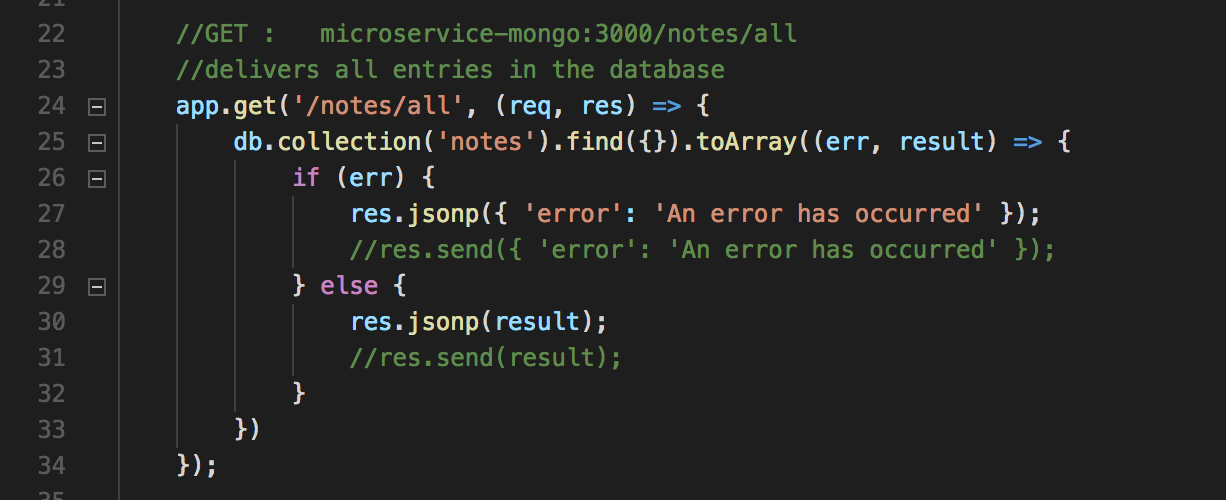
\includegraphics[height=.4\textwidth]{RoutesGetAll.png}
\vspace{3pt}
\caption{Schaubild\footnotemark}
\label{fig:blueant}
\end{figure}

Ein GET-Request an die "/notes/all" liefert alle in der Datenbank verzeichneten Einträge als Response.

\begin{figure}[h]
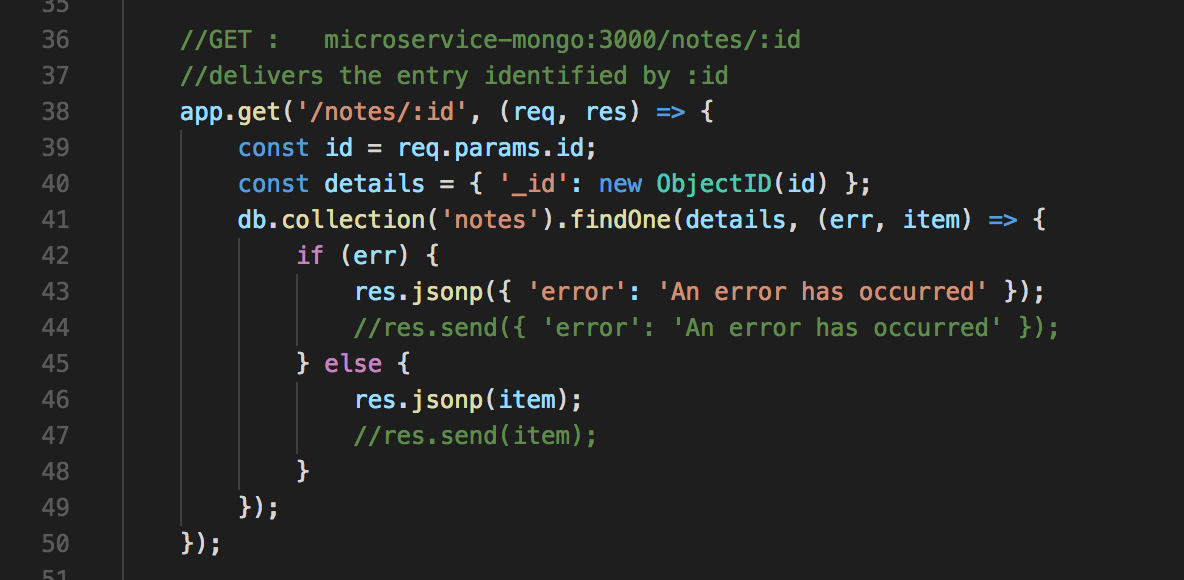
\includegraphics[height=.4\textwidth]{RoutesGetOne.png}
\vspace{3pt}
\caption{Schaubild\footnotemark}
\label{fig:blueant}
\end{figure}

Ein GET-Request an die "/notes/:id" liefert den Eintrag der Datenbank mit der angegebenen id als Response.

\begin{figure}[h]
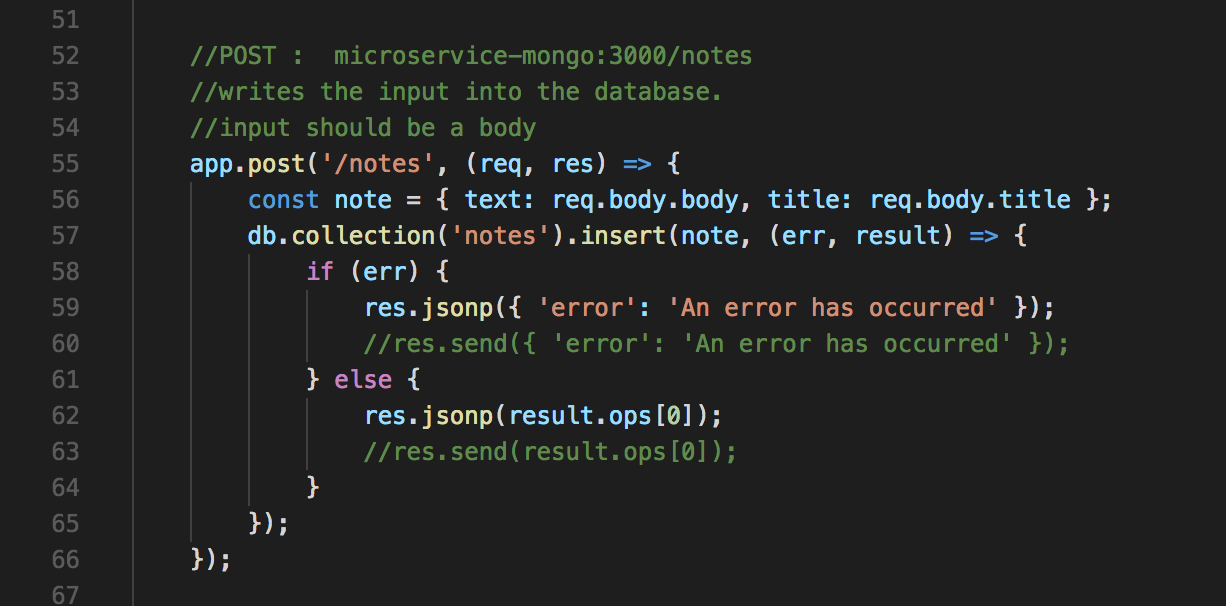
\includegraphics[height=.4\textwidth]{RoutesPost.png}
\vspace{3pt}
\caption{Schaubild\footnotemark}
\label{fig:blueant}
\end{figure}

Ein POST-Request an die "/notes" schreibt den Inhalt des gesendeten Bodys in die Datenbank.

\begin{figure}[h]
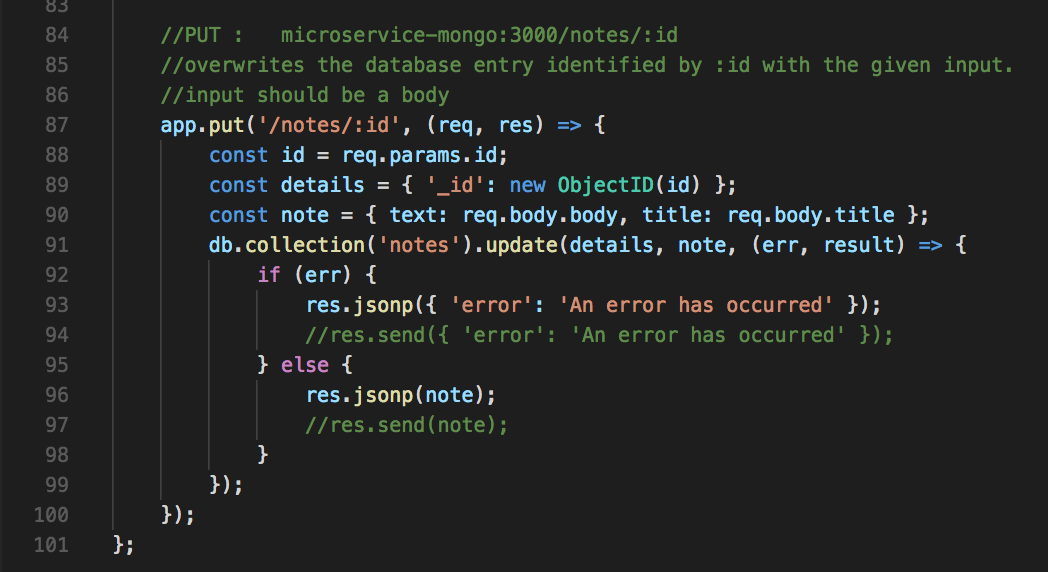
\includegraphics[height=.4\textwidth]{RoutesPut.png}
\vspace{3pt}
\caption{Schaubild\footnotemark}
\label{fig:blueant}
\end{figure}

Ein PUT-Request an die "/notes/:id" ersetzt den Inhalt des Datenbankeintrags mit der angegebenen Id mit dem Body des Requests.

\begin{figure}[h]
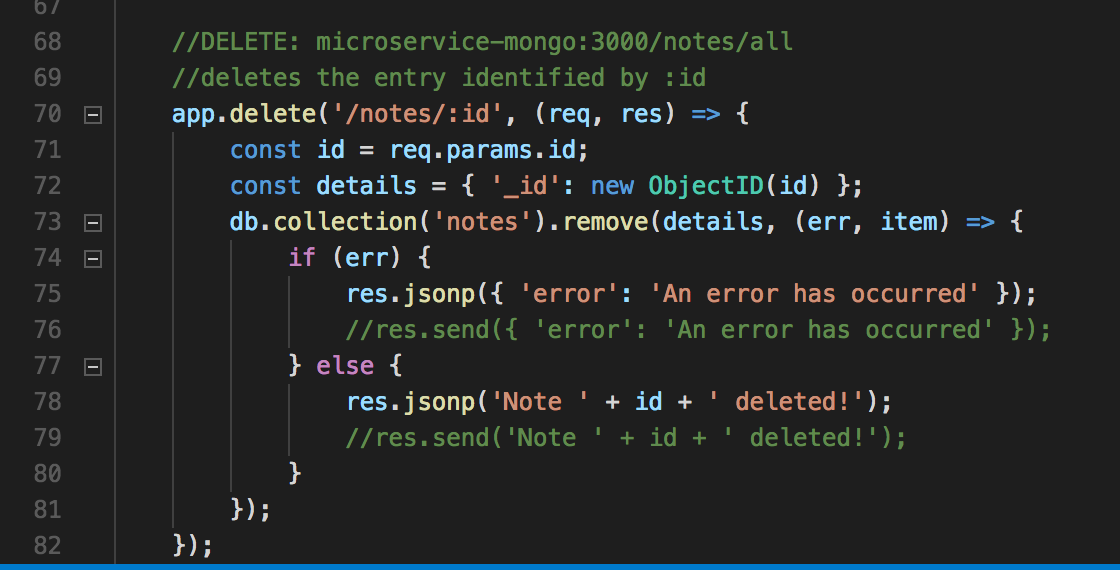
\includegraphics[height=.4\textwidth]{RoutesDelete.png}
\vspace{3pt}
\caption{Schaubild\footnotemark}
\label{fig:blueant}
\end{figure}

Ein DELETE-Request an die "/notes/:id" löscht den Datenbankeintrag mit der angegebenen Id.